%=====================
\chapter{Requirements}
%=====================
\label{chap:req:requirements}
This chapter describes a \gls{utility} that creates \Gls{wireshark} \glspl{dissector} from \Gls{c}
\gls{header} files. The \glspl{dissector} must interpret \gls{binary} representations of \Gls{c}
\glspl{struct}. In \autoref{sec:req:list} we give a high level overview of the
\gls{utility} and lists all the functional and non-function requirements, 
while \autoref{sec:req:usecases} provides use cases for the \gls{utility}, 
and \autoref{sec:prodbacklog} contains the complete product backlog.

%-----------------------------
\section{List of requirements}
%-----------------------------
\label{sec:req:list}

\subsection{Overview}
%-----------------
We are to create a \gls{utility} that allows \Gls{wireshark} to interpret the \gls{binary}
representations of \Gls{c}-language \glspl{struct}. While \Gls{c} \glspl{struct} seldom are exchanged
across networks, they are sometimes used in \gls{ipc}. The
purpose of the \gls{utility} described here is to provide \Gls{wireshark} with the
capability of automatically dissecting the \gls{binary} representation of a \Gls{c} \gls{struct},
as long as its definition is known.

The expected work flow for the \gls{utility} is to read one or more \Gls{c} \gls{header} files,
which contain \gls{struct} definitions, and output \Gls{wireshark} \glspl{dissector}, implemented
in \Gls{lua} scripts. A configuration file or source code annotations in the \gls{header}
files may be used when additional configuration is required.

\autoref{tab:req:func} lists the functional requirements, while
\autoref{tab:req:nonfunc} lists the non-functional requirements. Each
requirement have a priority (Pri) and a complexity (Cmp): \Gls{h}, 
\Gls{m} or \Gls{l} which is explained in \autoref{sec:req:priority} and
\autoref{sec:req:compl}.

\subsection{Prioritization}
%--------------------------
\label{sec:req:priority}
The team has, in cooperation with the customer, prioritized the requirements
in three categories:
\begin{inparaenum}[\itshape a\upshape)]
	\item High,
	\item Medium or
	\item Low.
\end{inparaenum} 

\begin{description}
	\item[High] Core functionality of the \gls{utility} that must be implemented.
	\item[Medium] Requirements that will improve the value of the \gls{utility}.
	\item[Low] Requirements that will not add much value to the \gls{utility}.
\end{description}

\subsection{Complexity}
%----------------------
\label{sec:req:compl}
The team has estimated the complexity for each requirement. We use the same
categories as for the prioritization of the requirements:
\begin{inparaenum}[\itshape a\upshape)]
	\item High,
	\item Medium or
	\item Low.
\end{inparaenum} 

\begin{description}
	\item[High] Functionality that seems difficult and non-trivial to create.
	\item[Medium] Functionality that seems time consuming but straight forward.
	\item[Low] Requirements that are trivial to implement.
\end{description}

%%%%%%%%%%%%%%%%%%%%%%%%%%%%%%%%%%%%
%%%%%%%%%%%%%%%%%%%%%%%%%%%%%%%%%%%%
%        OBS OBS OBS OBS
%
% These requirements are duplicated
% in many different locations,
% remember to update them all
%
% * product backlog
% * user stories
% * sprint 1 backlog
% * anywhere else?
%
%%%%%%%%%%%%%%%%%%%%%%%%%%%%%%%%%%%%
%%%%%%%%%%%%%%%%%%%%%%%%%%%%%%%%%%%%
\begin{table}[htbp] \footnotesize \center
\caption{Functional Requirements\label{tab:req:func}}
\noindent\makebox[\textwidth]{%
\begin{tabularx}{1.2\textwidth}{l X c c}
	\toprule
	ID & Description & Pri. & Cmp. \\
	\midrule
	FR1 & The \gls{utility} must be able to read basic \Gls{c} language \gls{struct} definitions from \Gls{c} \gls{header} files & \Gls{h} & \\
	FR1-A & The \gls{utility} must support the following basic data types: \gls{int}, \gls{float}, \gls{char} and \gls{boolean} & \Gls{h} & \Gls{l} \\
	FR1-B & The \gls{utility} must support \glspl{member} of type \gls{enum} & \Gls{h} & \Gls{l} \\
	FR1-C & The \gls{utility} must support \glspl{member} of type \gls{struct} & \Gls{h} & \Gls{m} \\
	FR1-D & The \gls{utility} must support \glspl{member} of type \gls{union} & \Gls{m} & \Gls{m} \\
	FR1-E & The \gls{utility} must support \glspl{member} of type \gls{array} & \Gls{h} & \Gls{m} \\
	FR1-F & The \gls{utility} should detect \glspl{struct} with the same name, and report it as an error & \Gls{m} & \Gls{l} \\
	\midrule
	FR2 & The \gls{utility} must be able to generate \Gls{lua} \glspl{dissector} for \Gls{wireshark} for the \gls{binary} representation of \Gls{c} \gls{struct} & \Gls{h} & \\
	FR2-A & The \gls{dissector} shall be able to display simple \glspl{struct} & \Gls{h} & \Gls{l} \\
	FR2-B & The \gls{dissector} shall be able to support \glspl{struct} within \glspl{struct} & \Gls{m} & \Gls{m} \\
	FR2-C & The \gls{dissector} must support \Gls{wireshark}'s built-in filter and search on attributes & \Gls{h} & \Gls{l} \\
	FR2-D & The \gls{dissector} shall be able to recognize invalid values for a \gls{struct} \gls{member} & \Gls{l} & \Gls{l} \\
	\midrule
	FR3 & The \gls{utility} must support \Gls{c} \gls{preprocessor} directives and macros & \Gls{h} & \\
	FR3-A & The \gls{utility} shall support \gls{include} & \Gls{h} & \Gls{l} \\
	FR3-B & The \gls{utility} shall support \gls{define} and \gls{if} & \Gls{h} & \Gls{l} \\
	FR3-C & The \gls{utility} shall support \verb+WIN32+, \verb+_WIN32+, \verb+_WIN64+, \verb+__sparc__+, \verb+__sparc+ and \verb+sun+ & \Gls{m} & \Gls{h} \\
	\midrule
	FR4 & The \gls{utility} must support user configuration & \Gls{m} & \\
	FR4-A & Configuration must support valid ranges for \gls{struct} \glspl{member} & \Gls{l} & \Gls{l} \\
	FR4-B & Configuration must support custom \Gls{lua} files for specific \glspl{protocol} & \Gls{h} & \Gls{h} \\
	FR4-C & Configuration must support custom handling of specific data types & \Gls{l} & \Gls{m} \\
	FR4-D & Configuration must support specifying the ID of \glspl{dissector} & \Gls{h} & \Gls{l} \\
	FR4-E & Configuration must support various trailers (other registered \gls{protocol}) & \Gls{l} & \Gls{h} \\
	FR4-F & Configuration must support integer \glspl{member} which represent enumerated named value & \Gls{m} & \Gls{l} \\	
	FR4-G & Configuration must support \glspl{member} which are \gls{bit string} & \Gls{m} & \Gls{l} \\
	\midrule
	FR5 & The \glspl{dissector} must be able to handle \gls{binary} input which size and \gls{endian} depends on originating platform & \Gls{m} & \\
	FR5-A & Flags must be specified in configuration for each platform & \Gls{m} & \Gls{m} \\
	FR5-B & Generate \glspl{dissector} with correct alignment depending on platform & \Gls{m} & \Gls{m} \\
	FR5-C & Generate \glspl{dissector} which support both little and big \gls{endian} platforms & \Gls{h} & \Gls{m} \\
	FR5-D & Generate \glspl{dissector} which support different sizes depending on platforms & \Gls{m} & \Gls{h} \\
	\midrule
	FR6 & The \gls{utility} shall support parameters from command line & \Gls{h} & \\
	FR6-A & Command line shall support parameter for \Gls{c} \gls{header} file & \Gls{h} & \Gls{l} \\
	FR6-B & Command line shall support parameter for configuration file & \Gls{h} & \Gls{l} \\
	FR6-C & Command line shall support batch processing of \Gls{c} \gls{header} and configuration files & \Gls{l} & \Gls{m} \\
	FR6-D & When running \gls{batch mode}, \glspl{dissector} that already are generated, shall not be regenerated, if the source are not modified since last run & \Gls{l} & \Gls{m} \\
	\midrule
	FR7 & Fetch configuration directly from source code & ? & ? \\
	FR7-A & Use Doxygen comments for strut members as "Description" & - & \\
	\bottomrule
\end{tabularx}}
\end{table}

\begin{table}[htbp] \footnotesize \center
\caption{Non-Functional Requirements\label{tab:req:nonfunc}}
\noindent\makebox[\textwidth]{%
\begin{tabularx}{1.2\textwidth}{l X c c}
	\toprule
	ID & Description & Pri. & Cmp. \\
	\midrule
	NR1 & The \gls{utility} shall be able to run on latest Windows and \Gls{Solaris} operating system & \Gls{m} & \Gls{l} \\
	\addlinespace
	NR2 & The \gls{dissector} shall be able to run on Windows \gls{x86}, Windows \gls{x86-64}, \Gls{Solaris} \gls{x86}, \Gls{Solaris} \gls{x86-64} and \Gls{Solaris} \gls{asparc} & \Gls{m} & \Gls{m} \\
	\addlinespace
	NR3 & The \gls{utility} shall only have a command line user interface. No \Gls{gui} \& clicking! & \Gls{h} & \Gls{l} \\
	\addlinespace
	NR4 & The \gls{utility} must have sufficient documentation to allow a person, with no prior knowledge of the system or \Gls{wireshark}, to be able to use it to generate \Gls{lua} \glspl{dissector} after five hours of reading & \Gls{m} & \Gls{m} \\
	\addlinespace
	NR5 & The \gls{utility} must have sufficient documentation to allow a person, with prior knowledge of \Gls{wireshark}, to be able to use it to generate \Gls{lua} \glspl{dissector} after one hour of reading & \Gls{m} & \Gls{m} \\
	\addlinespace
	NR6 & The \gls{utility} must have sufficient documentation to allow a person, already proficient with the system, to be able to extend its functionality after Y hours of reading & \Gls{m} & \Gls{m} \\
	\addlinespace
	NR7 & The \gls{utility} code should follow standard python coding convention as specified by PEP8 and try to follow python style guidelines defined by PEP20 & \Gls{h} & \Gls{l} \\
	\addlinespace
	NR8 & All Python modules, classes, functions and methods in the \gls{utility} should have docstrings which explains their code & \Gls{l} & \Gls{l} \\
	\bottomrule
\end{tabularx}}
\end{table}

%------------------
\section{Use Cases}d
%------------------
\label{sec:req:usecases}
This sections contains use case diagrams for our two actors, and detailed
textual use cases for these diagrams.

\subsection{Actors}
%------------------
An actor specifies a role played by an external person or thing that interact
with our \gls{utility}. We have three types of actors to consider. First is the
primary actor, which in our case is the user of our \gls{utility}. He who feeds it a
\Gls{c} file to generate \glspl{dissector}. A secondary actor is someone who configures our
\gls{utility} to change the output of it. Finally, we have an offstage actor, which
does not use our \gls{utility} himself, but uses the outputted \glspl{dissector} in \Gls{wireshark}.

We have defined two use case actors for our \gls{utility}. The customer has specified
that the offstage actor, called administrator, is the most important actor.
\begin{description}
	\item[Developer] User of the generated \Gls{wireshark} \glspl{dissector}, offstage actor
	\item[Administrator] User and configurer of \gls{utility}, primary and secondary actor
\end{description}

\subsection{Use Case Diagrams}
%-----------------------------
\hyperref[fig:req:ucadm]{Figure \ref*{fig:req:ucadm}} shows the use case
diagram for the administrator, and \autoref{fig:req:ucdev} is the use case
diagram for the developer.
\begin{figure}[htbp]
	\center
	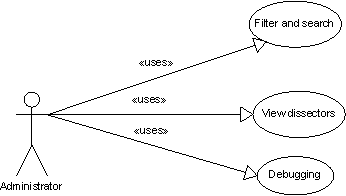
\includegraphics[width=0.8\textwidth]{./planning/img/administrator}
	\caption{Use Case Diagram: Administrator\label{fig:req:ucadm}}
\end{figure}

\begin{figure}[htbp]
	\center
	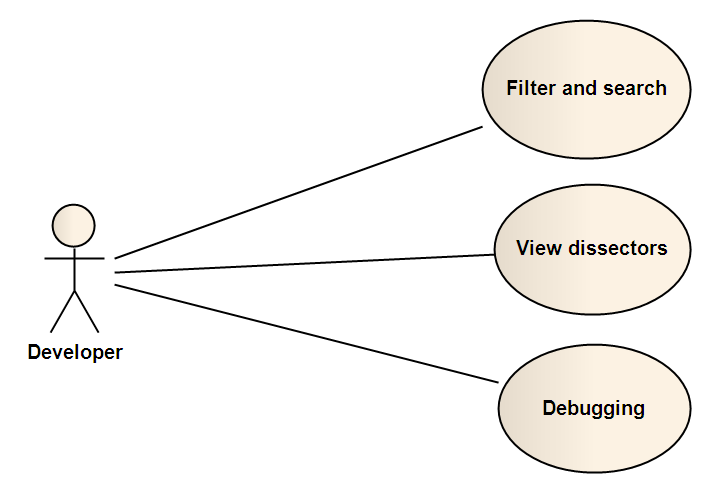
\includegraphics[width=0.8\textwidth]{./planning/img/developer}
	\caption{Use Case Diagram: Developer\label{fig:req:ucdev}}
\end{figure}

%Removed for pre-delivery
%\subsection{Textual Use Cases}
%-----------------------------
%TODO!!!

